%% LyX 2.3.4.2 created this file.  For more info, see http://www.lyx.org/.
%% Do not edit unless you really know what you are doing.
\documentclass[english,dvipsnames,aspectratio=169]{beamer}
\usepackage{mathptmx}
\usepackage{eulervm}
\usepackage[T1]{fontenc}
\usepackage[latin9]{inputenc}
\usepackage{babel}
\usepackage{amstext}
\usepackage{amssymb}
\usepackage{graphicx}
\usepackage{ifthen}
\usepackage{xcolor}
\usepackage{booktabs}
\usepackage{xspace}
\usepackage{tikz}
\usetikzlibrary{tikzmark}
\usetikzlibrary{calc}
\usepackage{pgfplots}
%\pgfplotsset{compat=1.17}
\usepackage{booktabs}
\usepackage{xpatch}

\xpatchcmd{\itemize}
  {\def\makelabel}
  {\ifnum\@itemdepth=1\relax
     \setlength\itemsep{2ex}% separation for first level
   \else
     \ifnum\@itemdepth=2\relax
       \setlength\itemsep{1ex}% separation for second level
     \else
       \ifnum\@itemdepth=3\relax
         \setlength\itemsep{0.5ex}% separation for third level
   \fi\fi\fi\def\makelabel
  }
 {}
 {}

\ifx\hypersetup\undefined
  \AtBeginDocument{%
    \hypersetup{unicode=true,pdfusetitle,
 bookmarks=true,bookmarksnumbered=false,bookmarksopen=false,
 breaklinks=false,pdfborder={0 0 0},pdfborderstyle={},backref=false,colorlinks=true,
 allcolors=NYUPurple,urlcolor=LightPurple}
  }
\else
  \hypersetup{unicode=true,pdfusetitle,
 bookmarks=true,bookmarksnumbered=false,bookmarksopen=false,
 breaklinks=false,pdfborder={0 0 0},pdfborderstyle={},backref=false,colorlinks=true,
 allcolors=NYUPurple,urlcolor=LightPurple}
\fi

\makeatletter

%%%%%%%%%%%%%%%%%%%%%%%%%%%%%% LyX specific LaTeX commands.
%% Because html converters don't know tabularnewline
\providecommand{\tabularnewline}{\\}

%%%%%%%%%%%%%%%%%%%%%%%%%%%%%% Textclass specific LaTeX commands.
% this default might be overridden by plain title style
\newcommand\makebeamertitle{\frame{\maketitle}}%
% (ERT) argument for the TOC
\AtBeginDocument{%
  \let\origtableofcontents=\tableofcontents
  \def\tableofcontents{\@ifnextchar[{\origtableofcontents}{\gobbletableofcontents}}
  \def\gobbletableofcontents#1{\origtableofcontents}
}

%%%%%%%%%%%%%%%%%%%%%%%%%%%%%% User specified LaTeX commands.
\usetheme{CambridgeUS} 
\beamertemplatenavigationsymbolsempty


% Set Color ==============================
\definecolor{NYUPurple}{RGB}{87,6,140}
\definecolor{LightPurple}{RGB}{165,11,255}


\setbeamercolor{title}{fg=NYUPurple}
\setbeamercolor{frametitle}{fg=NYUPurple}

\setbeamercolor{background canvas}{fg=NYUPurple, bg=white}
\setbeamercolor{background}{fg=black, bg=NYUPurple}

\setbeamercolor{palette primary}{fg=black, bg=gray!30!white}
\setbeamercolor{palette secondary}{fg=black, bg=gray!20!white}
\setbeamercolor{palette tertiary}{fg=gray!20!white, bg=NYUPurple}

\setbeamertemplate{headline}{}
\setbeamerfont{itemize/enumerate body}{}
\setbeamerfont{itemize/enumerate subbody}{size=\normalsize}
\setbeamerfont{itemize/enumerate subsubbody}{size=\normalsize}

\setbeamercolor{parttitle}{fg=NYUPurple}
\setbeamercolor{sectiontitle}{fg=NYUPurple}
\setbeamercolor{sectionname}{fg=NYUPurple}
\setbeamercolor{section page}{fg=NYUPurple}
%\setbeamercolor{description item}{fg=NYUPurple}
%\setbeamercolor{block title}{fg=NYUPurple}

\setbeamertemplate{blocks}[rounded][shadow=false]
\setbeamercolor{block body}{bg=normal text.bg!90!NYUPurple}
\setbeamercolor{block title}{bg=NYUPurple!30, fg=NYUPurple}



\AtBeginSection[]{
  \begin{frame}
  \vfill
  \centering
\setbeamercolor{section title}{fg=NYUPurple}
 \begin{beamercolorbox}[sep=8pt,center,shadow=true,rounded=true]{title}
    \usebeamerfont{title}\usebeamercolor[fg]{title}\insertsectionhead\par%
  \end{beamercolorbox}
  \vfill
  \end{frame}
}

\makeatother

\setlength{\parskip}{\medskipamount} 

\input ../macros

\begin{document}
\input ../rosenberg-macros

\title[DS-GA 1003]{Subgradient Descent}
\author{He He}
\date{Feb 23, 2021}
\institute{CDS, NYU}

\makebeamertitle
\mode<article>{Just in article version}

\begin{frame}{SVM Optimization Problem (no intercept)}
\begin{itemize}
\item SVM objective function:
\[
    J(w)=\frac{1}{n}\sum_{i=1}^{n}\max\left(0,1-{y_{i}w^{T}x_{i}}\right)+\lambda||w||^{2}.
\]

\item Not differentiable... but let's think about gradient descent anyway.
\item Hinge loss: $\ell(m)=\max(0,1-m)$
%\item Derivative of hinge loss $\ell(m)=\max(0,1-m)$:
%\[
%\ell'(m)=\begin{cases}
%0 & m>1\\
%-1 & m<1\\
%\text{undefined} & m=1
%\end{cases}
%\]
\end{itemize}
\begin{eqnarray*}
\del_{w}J(w) & = & \del_{w}\left(\frac{1}{n}\sum_{i=1}^{n}\ell\left(y_{i}w^{T}x_{i}\right)+\lambda||w||^{2}\right)\\
 & = & \frac{1}{n}\sum_{i=1}^{n}\del_{w}\ell\left(y_{i}w^{T}x_{i}\right)+2\lambda w\\
% & = & \begin{cases}
%\frac{1}{n}\sum_{i:y_{i}w^{T}x_{i}<1}\left(-y_{i}x_{i}\right)+2\lambda w & \text{all }y_{i}w^{T}x_{i}\neq1\\
%\text{undefined} & \text{otherwise}
%\end{cases}
\end{eqnarray*}
\end{frame}

\begin{frame}{``Gradient'' of SVM Objective}
    \begin{itemize}
\item Derivative of hinge loss $\ell(m)=\max(0,1-m)$:
$$
\ell'(m)=\begin{cases}
0 & m>1\\
-1 & m<1\\
\text{undefined} & m=1
\end{cases}
$$

\item By chain rule, we have 
\begin{eqnarray*}
\del_{w}\ell\left(y_{i}w^{T}x_{i}\right) & = & \ell'\left(y_{i}w^{T}x_{i}\right)y_{i}x_{i}\\
& = & \begin{cases}
0 & y_{i}w^{T}x_{i}>1\\
-y_{i}x_{i} & y_{i}w^{T}x_{i}<1\\
\text{undefined} & y_{i}w^{T}x_{i}=1
\end{cases}
\end{eqnarray*}
\end{itemize}
\end{frame}

\begin{frame}{``Gradient'' of SVM Objective}

\begin{eqnarray*}
\del_{w}\ell\left(y_{i}w^{T}x_{i}\right) & = & \begin{cases}
0 & y_{i}w^{T}x_{i}>1\\
-y_{i}x_{i} & y_{i}w^{T}x_{i}<1\\
\text{undefined} & y_{i}w^{T}x_{i}=1
\end{cases}
\end{eqnarray*}

So 
    \vspace{-2ex}
\begin{eqnarray*}
\del_{w}J(w) & = & \del_{w}\left(\frac{1}{n}\sum_{i=1}^{n}\ell\left(y_{i}w^{T}x_{i}\right)+\lambda||w||^{2}\right)\\
 & = & \frac{1}{n}\sum_{i=1}^{n}\del_{w}\ell\left(y_{i}w^{T}x_{i}\right)+2\lambda w\\
 & = & \begin{cases}
\frac{1}{n}\sum_{i:y_{i}w^{T}x_{i}<1}\left(-y_{i}x_{i}\right)+2\lambda w & \text{all }y_{i}w^{T}x_{i}\neq1\\
\text{undefined} & \text{otherwise}
\end{cases}
\end{eqnarray*}
\end{frame}

\begin{frame}{Gradient Descent on SVM Objective?}
\begin{itemize}
\item The gradient of the SVM objective is
\[
\del_{w}J(w)=\frac{1}{n}\sum_{i:y_{i}w^{T}x_{i}<1}\left(-y_{i}x_{i}\right)+2\lambda w
\]
 when $y_{i}w^{T}x_{i}\neq1$ for all $i$, and \hl{otherwise
is undefined}.
\end{itemize}

Potential arguments for why we shouldn't care about the points of
nondifferentiability:\\
\begin{itemize}
\item If we start with a random $w$, will we ever hit exactly $y_{i}w^{T}x_{i}=1$?

\item If we did, could we perturb the step size by $\eps$ to miss such
a point?

\item Does it even make sense to check $y_{i}w^{T}x_{i}=1$ with floating
point numbers?
\end{itemize}
However, would gradient descent work if the objective is not differentiable?
\end{frame}

\section{Subgradient}
\begin{frame}{First-Order Condition for Convex, Differentiable Function}

\begin{itemize}
\item Suppose $f:\reals^{d}\to\reals$ is \hl{convex} and \hl{differentiable}
Then for any $x,y\in\reals^{d}$
\[
f(y)\ge f(x)+\del f(x)^{T}(y-x)
\]


\item The linear approximation to $f$ at $x$ is a \hl{global underestimator
}of $f$:
\begin{center}
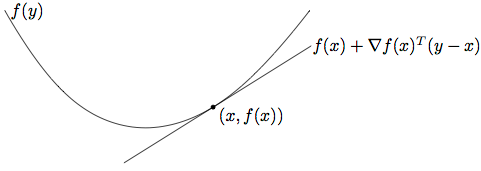
\includegraphics[width=0.5\columnwidth]{figures/BVFig3.2-convexTangent}
\par\end{center}
\item This implies that 
if $\del f(x)=0$ then $x$ is a global minimizer of $f$.
\end{itemize}
\let\thefootnote\relax\footnotetext{\tiny{Figure from Boyd \& Vandenberghe Fig. 3.2; Proof in Section 3.1.3 }}
\end{frame}

\begin{frame}{Subgradients}
\begin{definition}
    A vector $g\in\reals^{d}$ is a \textbf{subgradient} of a \emph{convex} function $f:\reals^{d}\to\reals$
at $x$ if for all $z$, 
$$
f(z)\ge f(x)+g^{T}(z-x).
$$
\end{definition}

\begin{center}
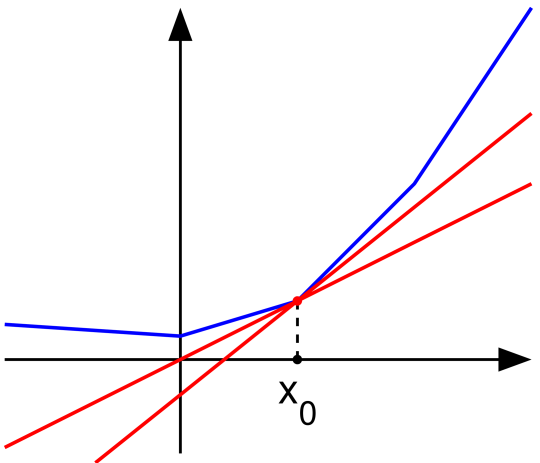
\includegraphics[height=0.4\textheight]{figures/Subderivative_illustration}
\par\end{center}

Blue is a graph of $f(x)$. \\
Each red line $x\mapsto f(x_{0})+g^{T}\left(x-x_{0}\right)$ is a
    \hl{global lower bound} on $f(x)$.
\end{frame}

\begin{frame}
    {Properties}
\begin{definitions}
\begin{itemize}
\item The set of all subgradients at $x$ is called the \textbf{subdifferential}:
$\partial f(x)$ 
\item $f$ is \textbf{subdifferentiable} at $x$ if $\exists$ at least
one subgradient at $x$. 
\end{itemize}
\end{definitions}

For convex functions:\\
    \begin{itemize}
        \setlength\itemsep{1ex}
\item $f$ is differentiable at $x$ iff $\partial f(x)=\left\{ \del f(x)\right\}$.
\item Subdifferential is always non-empty ($\partial f(x)=\emptyset \implies f$ is not convex)
\item $x$ is the global optimum iff $0\in\partial f(x)$.
    \end{itemize}

    For non-convex functions:\\
    \begin{itemize}
        \item The subdifferential may be an empty set (no global underestimator).
    \end{itemize}
\end{frame}

\begin{frame}{Subdifferential of Absolute Value}
\begin{itemize}
\item Consider $f(x)=\left|x\right|$

\end{itemize}
\let\thefootnote\relax\footnotetext{\tiny{Boyd EE364b: Subgradients Slides}}

\begin{center}
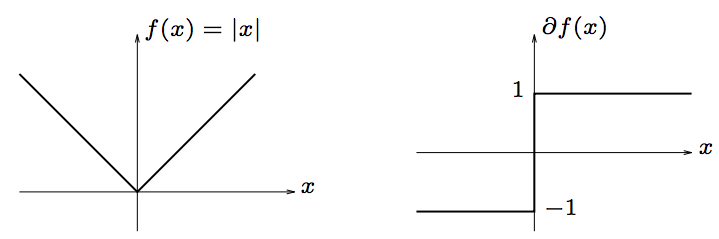
\includegraphics[width=0.8\columnwidth]{figures/subgradient-absolute-value}
\par\end{center}
\begin{itemize}
\item Plot on right shows $\left\{ (x,g)\mid x\in\reals,\;g\in\partial f(x)\right\} $ 
\end{itemize}
\end{frame}


\begin{frame}{Subgradients of $f(x_{1},x_{2})=\left|x_{1}\right|+2\left|x_{2}\right|$}
    \begin{columns}

        \begin{column}{0.6\textwidth}
\begin{itemize}
\item Let's find the subdifferential of $f(x_{1},x_{2})=\left|x_{1}\right|+2\left|x_{2}\right|$
at $\left(3,0\right)$.
\end{itemize}

\begin{itemize}
\item First coordinate of subgradient must be $1$, from $\left|x_{1}\right|$
part (at $x_{1}=3$).
\end{itemize}

\begin{itemize}
\item Second coordinate of subgradient can be anything in $\left[-2,2\right]$.
\end{itemize}

\begin{itemize}
\item So graph of $h(x_{1},x_{2})=f(3,0)+g^{T}\left(x_{1}-3,x_{2}-0\right)$
is a global underestimate of $f(x_{1},x_{2})$, for any $g=\left(g_{1},g_{2}\right),$
where $g_{1}=1$ and $g_{2}\in[-2,2]$. 
\end{itemize}
    \end{column}
        \begin{column}{0.3\textwidth}
\begin{center}
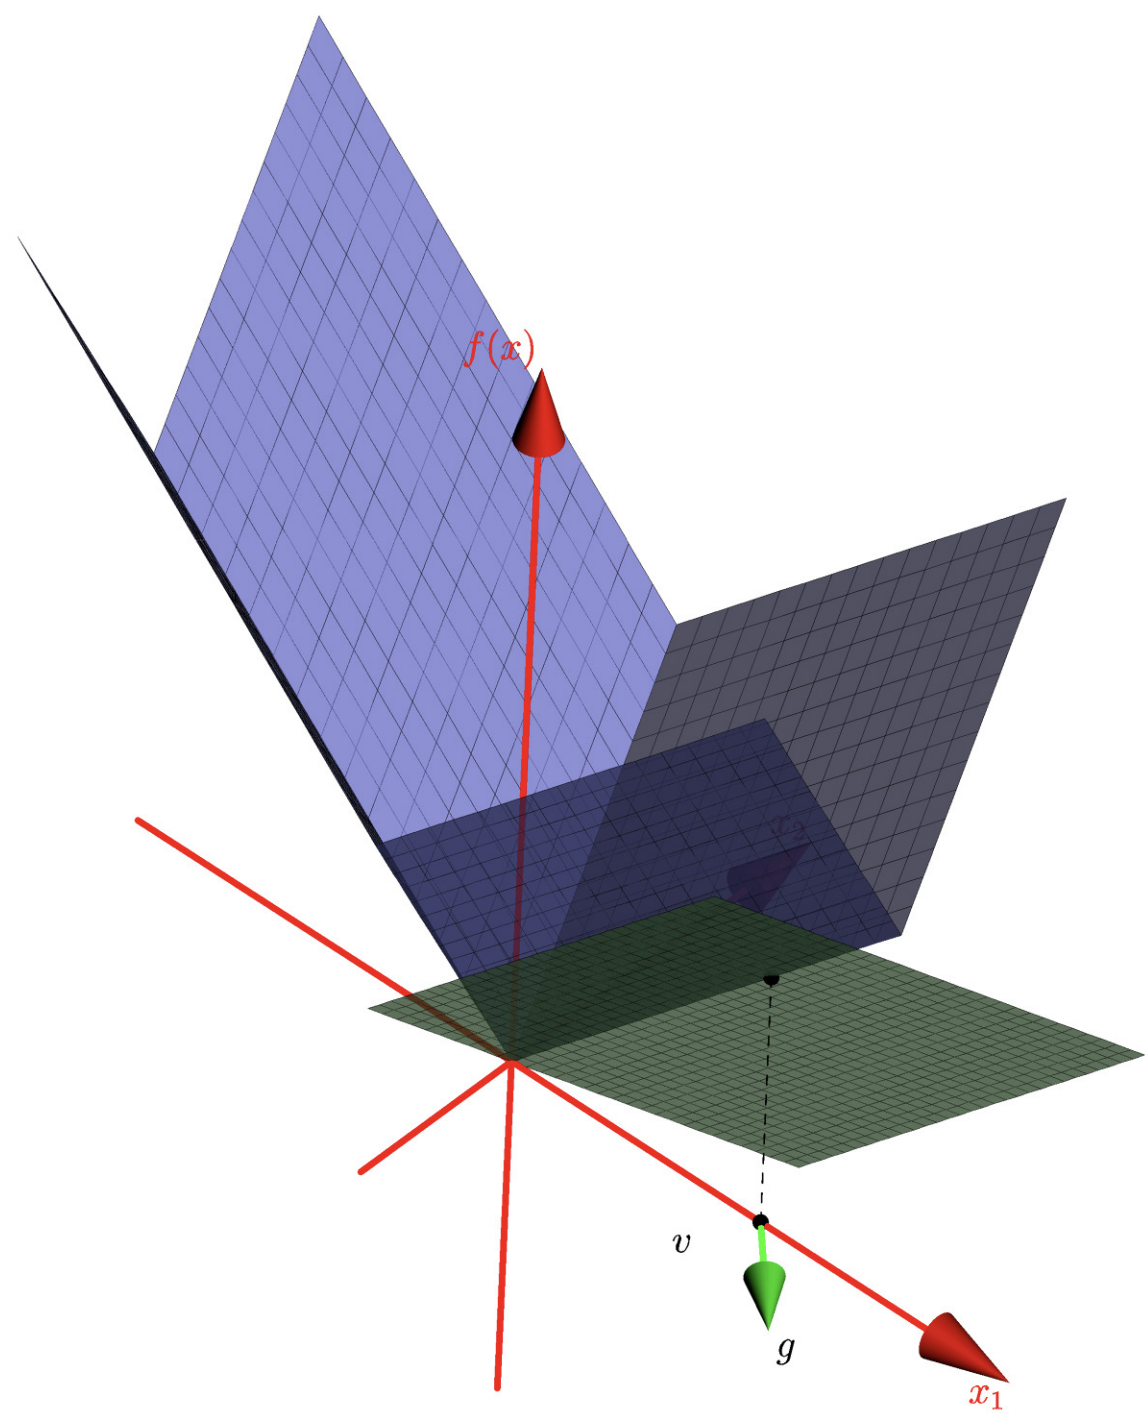
\includegraphics[height=0.75\textheight]{figures/underestimating-3d-plot-abs-x1-plus-2absx2}\let\thefootnote\relax\footnotetext{\tiny{Plot courtesy of Brett Bernstein.}} 
\par\end{center}
        \end{column}
    \end{columns}
\end{frame}

\begin{frame}{Subdifferential on Contour Plot}
\begin{center}
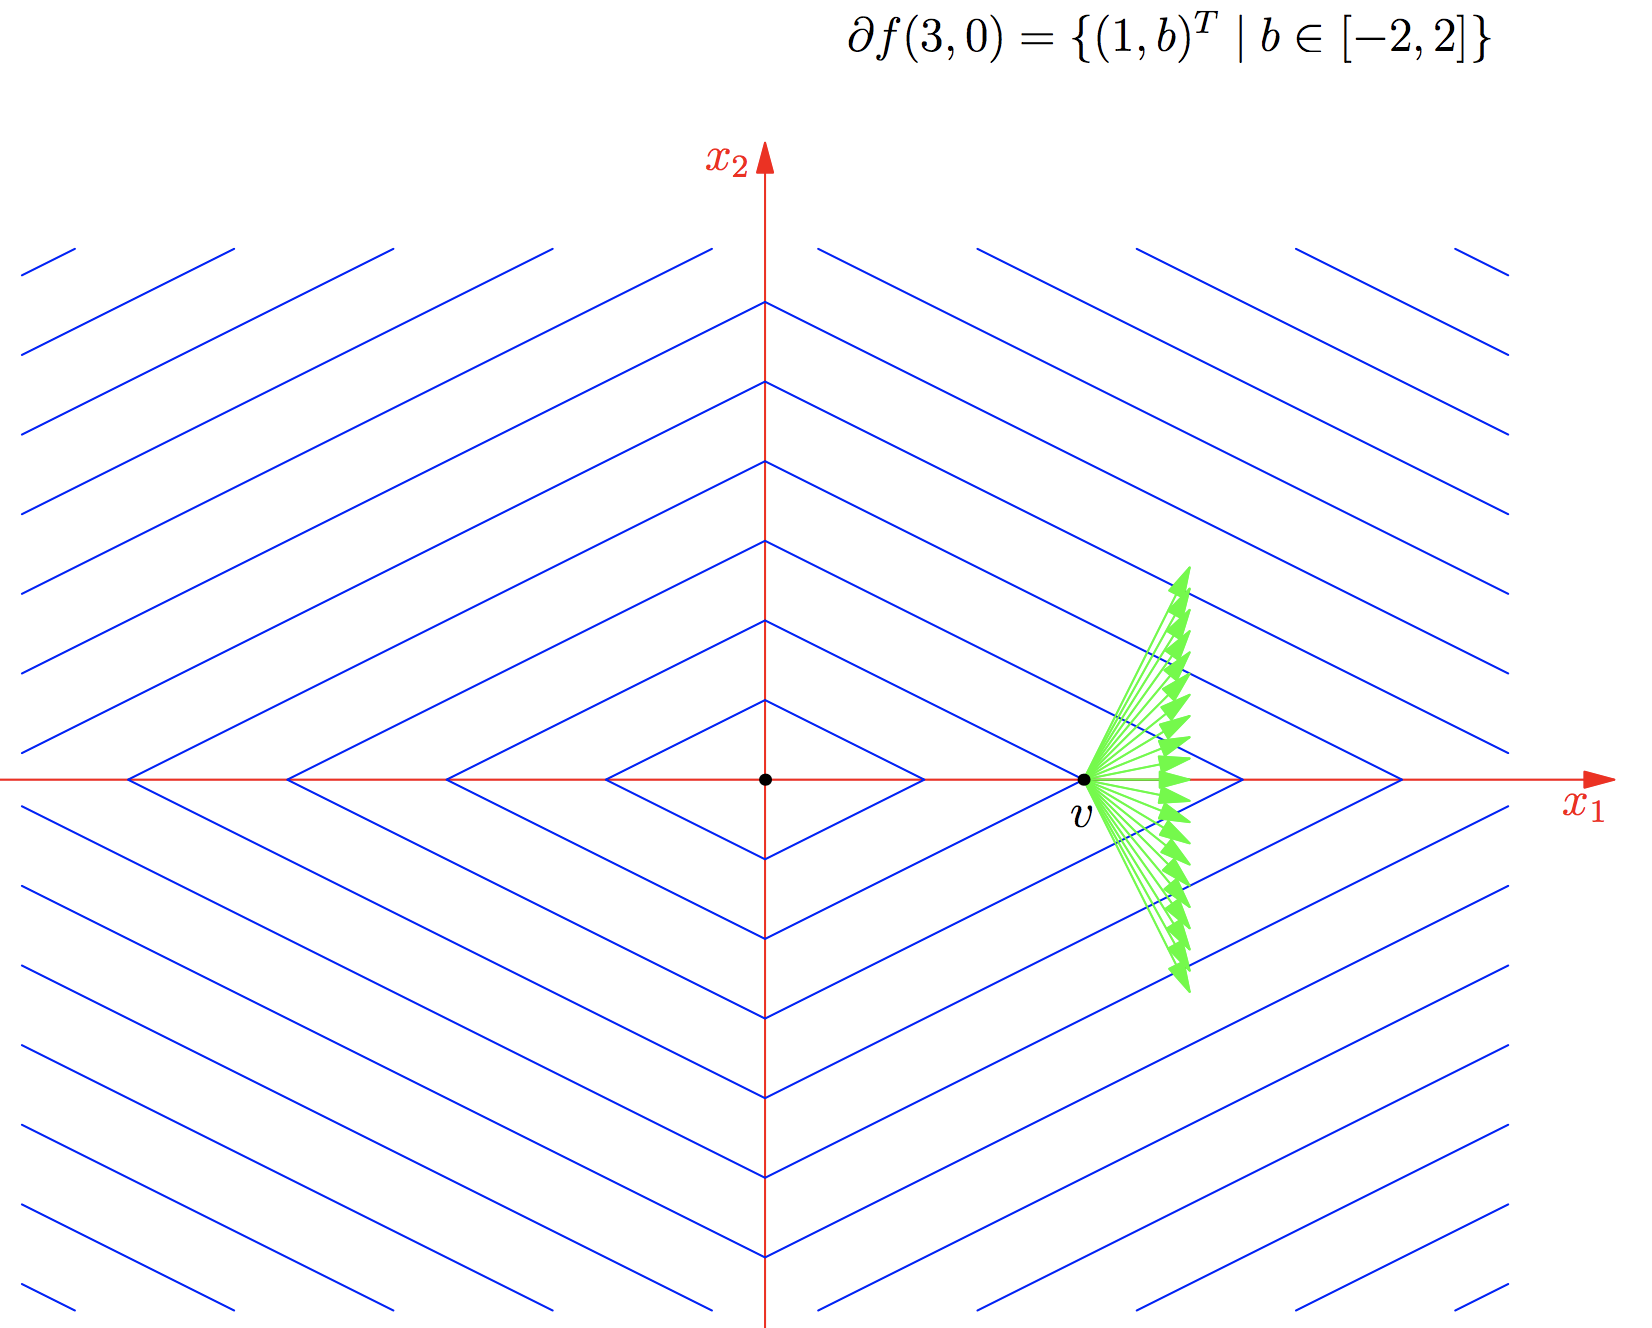
\includegraphics[height=0.6\textheight]{figures/subdiff-contour-plot-abs-x1-plus-2absx2}
\par\end{center}

\begin{center}
Contour plot of $f(x_{1},x_{2})=\left|x_{1}\right|+2\left|x_{2}\right|$,
with set of subgradients at $(3,0)$. .\let\thefootnote\relax\footnotetext{\tiny{Plot courtesy of Brett Bernstein.}}
\par\end{center}
\end{frame}

\begin{frame}
    {Basic Rules for Calculating Subdifferential}
    \begin{itemize}
        \item \head{Non-negative scaling}: $\partial \alpha f(x) = \alpha\partial f(x)$ for $(\alpha > 0)$
        \item \head{Summation}: $\partial(f_1(x) + f_2(x)) = d_1 + d_2$ for any $d_1\in\partial f_1$ and $d_2 \in\partial f_2$
        \item \head{Composing with affine functions}: $\partial f(Ax+b) = A^T\partial f(z)$ where $z=Ax+b$
        \item \head{max}: convex combinations of argmax gradients
            $$
            \partial \max(f_1(x), f_2(x)) =
            \begin{cases}
                \nabla f_1(x) & \text{if } f_1(x) > f_2(x), \\
                \nabla f_2(x) & \text{if } f_1(x) < f_2(x), \\
                \nabla \theta f_1(x) + (1-\theta)f_2(x) & \text{if } f_1(x) = f_2(x), \\
            \end{cases}
            $$
            where $\theta \in[0,1]$.
    \end{itemize}
\end{frame}

\section{Subgradient Descent}
\begin{frame}{Gradient orthogonal to level sets}
    We know that gradient points to the fastest ascent direction.
    What about subgradients?
\begin{center}
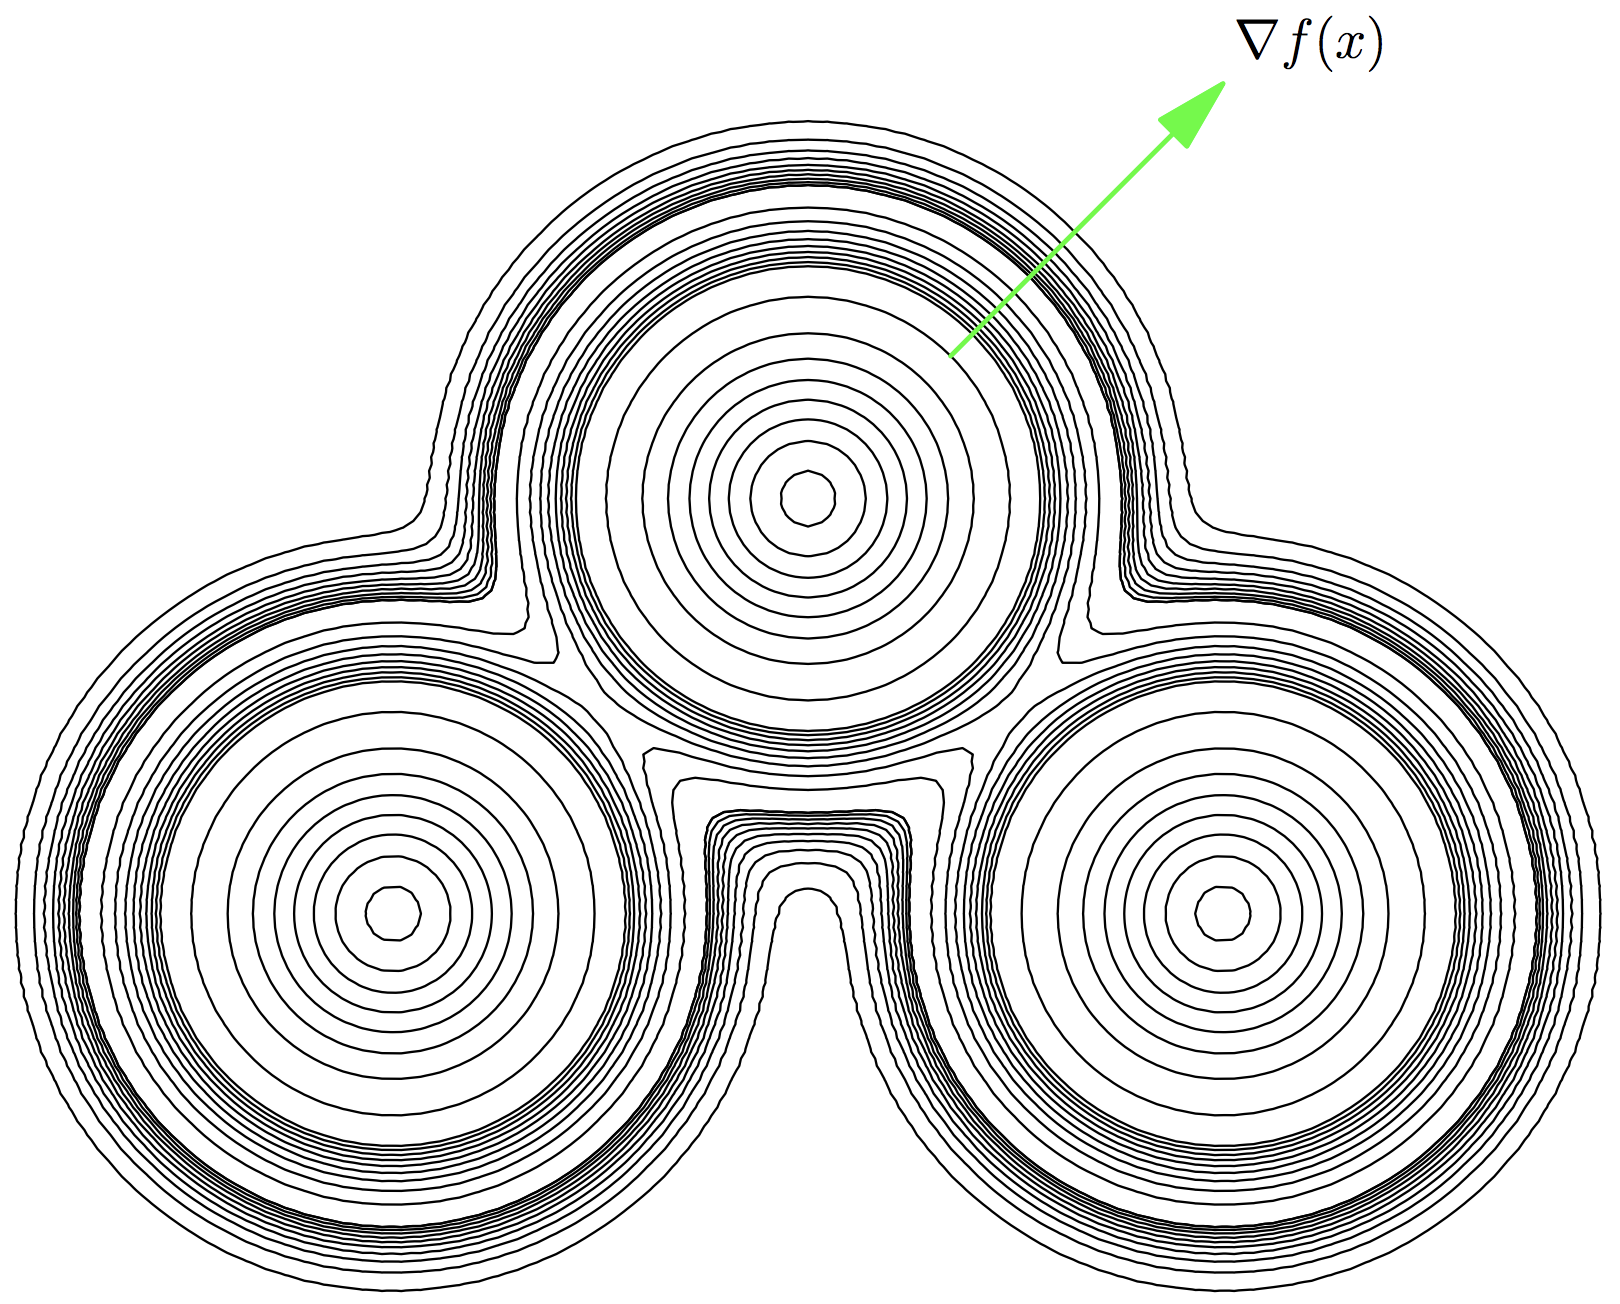
\includegraphics[height=0.6\textheight]{figures/grad-orthog-to-sublevel-sets}\let\thefootnote\relax\footnotetext{\tiny{Plot courtesy of Brett Bernstein.}}
\par\end{center}
\end{frame}

\begin{frame}{Contour Lines and Subgradients }
A hyperplane $H$ \textbf{supports} a set $S$ if $H$ intersects
$S$ and all of $S$ lies one one side of $H$.

    \head{Claim}: If $f:\reals^{d}\to\reals$ has subgradient $g$ at $x_{0}$, then
the hyperplane $H$ orthogonal to $g$ at $x_{0}$ must \textbf{support}
the level set $S=\left\{ x\in\reals^{d}\mid f(x)=f(x_{0})\right\} $. 

Proof:\\
\begin{itemize}
    \setlength\itemsep{1ex}
\item For any $y$, we have $f(y)\ge f(x_{0})+g^{T}(y-x_{0})$. (def
of subgradient)
\item If $y$ is strictly on side of $H$ that $g$ points in,
    \begin{itemize}
\item then $g^{T}\left(y-x_{0}\right)>0$.
\item So $f(y)>f(x_{0})$.
\item So $y$ is not in the level set $S$.
\end{itemize}
\item $\therefore$ All elements of $S$ must be on $H$ or on the $-g$
side of $H$.
\end{itemize}
\end{frame}

\begin{frame}{Subgradient of $f(x_{1},x_{2})=\left|x_{1}\right|+2\left|x_{2}\right|$ }
\begin{center}
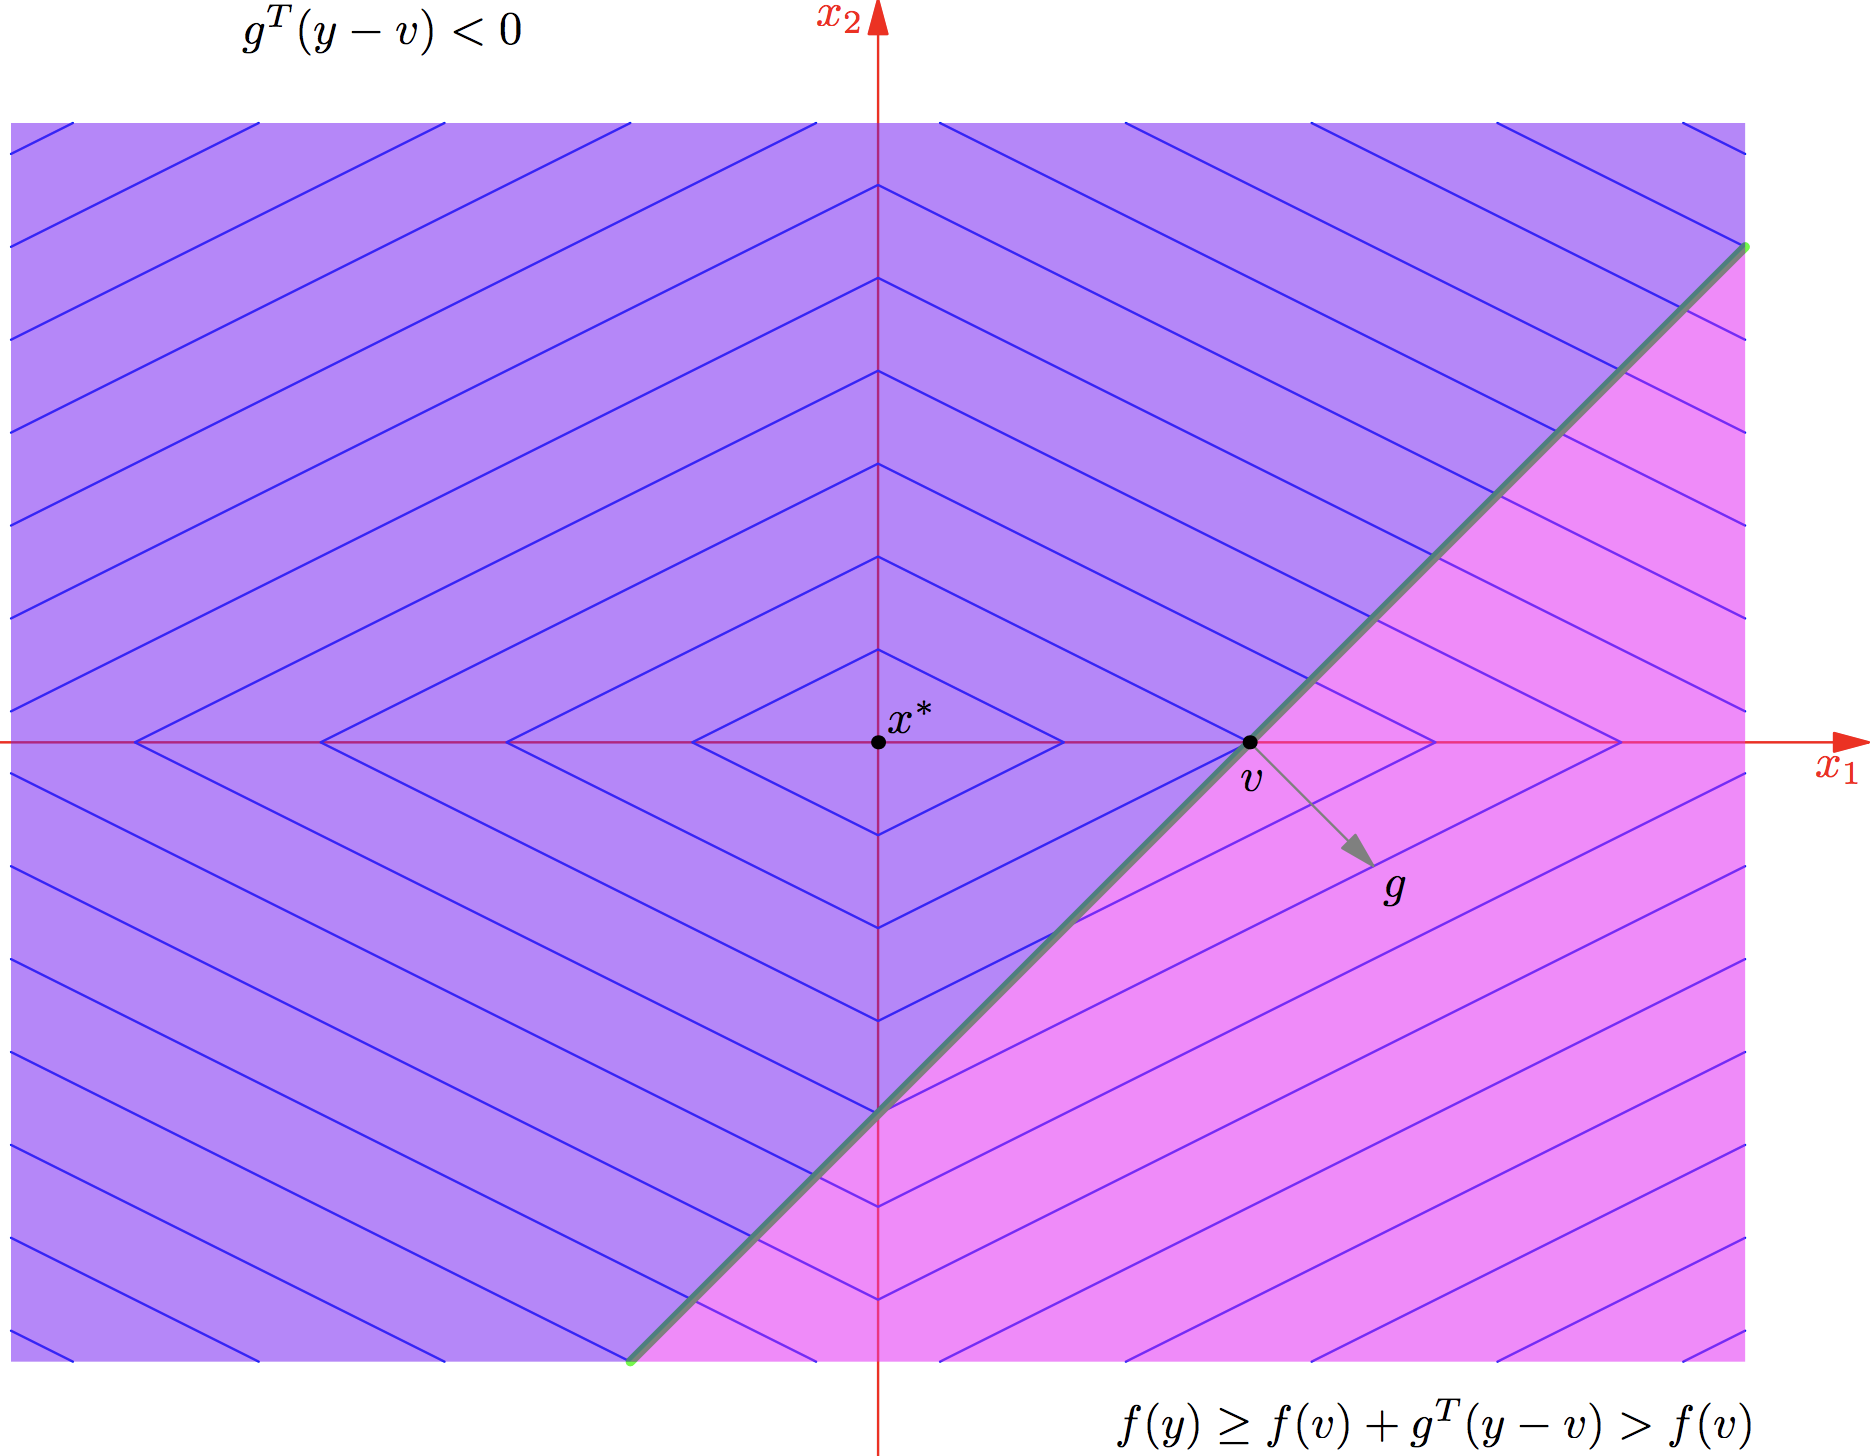
\includegraphics[height=0.6\textheight]{figures/contour-plot-abs-x1-plus-2absx2}\let\thefootnote\relax\footnotetext{\tiny{Plot courtesy of Brett Bernstein.}}
\par\end{center}
    \vspace{-1em}
\begin{itemize}
    \setlength\itemsep{1ex}
\item Points on $g$ side of $H$ have larger $f$-values than $f(x_{0})$.
(from proof)
\item But points on $-g$ side may \textbf{not }have smaller $f$-values. 
\item So $-g$ may \textbf{not} be a descent direction. (shown in figure)
\end{itemize}
\end{frame}

\begin{frame}
    {Subgradient Descent}
    \begin{itemize}
        \item Move along the negative subgradient:
            $$
            x^{t+1} = x^t - \eta g \quad \text{where } g\in\partial f(x^t) \text{ and } \eta > 0
            $$
        \item This can \al{increase} the objective but gets us \hl{closer to the minimizer} if $f$ is convex and $\eta$ is small enough:
            $$
            \|x^{t+1} - x^*\| < \|x^{t} - x^*\|
            $$
        \item Subgradients don't necessarily converge to zero as we get closer to $x^*$, so we need \al{decreasing step sizes}, e.g. $O(1/t)$ or $O(1/\sqrt{t})$.
        \item Subgradient methods are \al{slower} than gradient descent,
            e.g. ${\color{red}O(1/\epsilon^2)}$ vs $O(1/\epsilon)$ for convex functions.
    \end{itemize}
    \let\thefootnote\relax\footnotetext{\tiny{Based on \url{https://www.cs.ubc.ca/~schmidtm/Courses/5XX-S20/S4.pdf}}}
\end{frame}

\begin{frame}
    {Subgradient descent for SVM (HW3)}
SVM objective function:
    \vspace{-1em}
\[
    J(w)=\frac{1}{n}\sum_{i=1}^{n}\max\left(0,1-{y_{i}w^{T}x_{i}}\right)+\lambda||w||^{2}.
\]

    Pegasos: stochastic subgradient descent with step size $\eta_t = 1/(t\lambda)$
    \vspace{-1em}
    \begin{figure}
        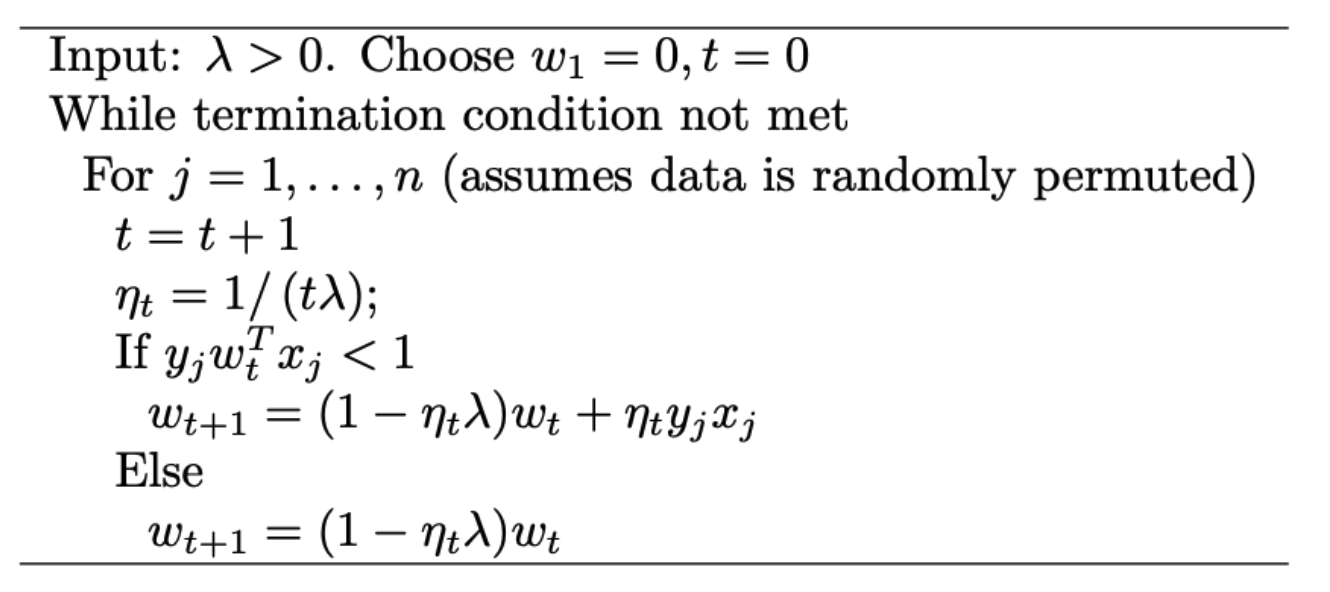
\includegraphics[height=0.5\textheight]{figures/pegasos}
    \end{figure}
\end{frame}

\begin{frame}
    {Summary}
    \begin{itemize}
        \item Subgradient: generalize gradient for non-differentiable convex functions
        \item Subgradient ``descent'':
            \begin{itemize}
                \item General method for non-smooth functions
                \item Simple to implement
                \item Slow to converge
            \end{itemize}
    \end{itemize}
\end{frame}

\end{document}
